\documentclass[11pt,a4paper]{article}
\usepackage[margin=20mm]{geometry}
\usepackage{amsmath,amssymb,booktabs,array,tikz,enumitem,hyperref}
\usetikzlibrary{arrows.meta,positioning}
\setlength{\parindent}{0pt}\setlength{\parskip}{6pt}
\newcommand{\question}[2]{\section*{#1: #2}}
\tikzset{v/.style={draw,circle,minimum size=10mm,align=center,inner sep=2pt},bf/.style={v,double},arr/.style={->,>=Stealth}}
\begin{document}
\begin{center}{\Large\bfseries Search Algorithms: Worked Answers}\\[4pt]BFS, DFS, Dijkstra, and A*\end{center}
\small Original questions: requirements/BFS-DFS-Dijkstra-Astar-homework.pdf, pp.\ 1--10.\normalsize

\question{BFS1 (p.\ 1)}{Number of states searched}
Use the initial board $\left[\begin{smallmatrix}2&8&3\\1&6&4\\7&\square&5\end{smallmatrix}\right]$. Number the root as depth 0, and exclude repeated states, including the immediate reversal of the previous move. The numbers of distinct states at depths 0 through 5 are:
\begin{center}\begin{tabular}{c|rrrrrr}\toprule
Depth $d$&0&1&2&3&4&5\\\midrule
States $N_d$&1&3&5&10&14&28\\\bottomrule
\end{tabular}\end{center}
The blank initially lies at an edge position, giving three first moves. Each corner blank has two legal moves, each edge blank has three, and the center blank has four. Excluding the move back to the parent gives the following layer calculation:
\begin{center}\begin{tabular}{c|rrr|r}\toprule
Depth&Corner blanks&Edge blanks&Center blanks&Total\\\midrule
0&0&1&0&1\\1&2&0&1&3\\2&0&5&0&5\\3&8&0&2&10\\4&0&14&0&14\\5&20&0&8&28\\\bottomrule\end{tabular}\end{center}
For example, depth 2 has $2(2-1)+(4-1)=5$ states; depth 3 has $5(3-1)=10$ states. Through depth 5, these generated configurations are distinct after parent reversals are excluded.

BFS examines every shallower layer before depth 5. With the question's assumption that half of depth 5 is searched, the total is
\[
N=1+3+5+10+14+\frac{28}{2}=\boxed{47\text{ states}}.
\]
This counts the root and the goal among the states examined. The printed label ``27'' beside the goal is a diagram label, not a BFS examination count. The answer uses the stated halfway assumption; it is not a claim about a particular implementation's goal-test ordering or total generated queue entries.

\newpage
\question{DFS1 (p.\ 2)}{Search tree and backtracking}
Follow the recursive order illustrated on the question sheet:
\[
u\to v\to t\to s,\qquad\text{return to }t,\qquad t\to r\to w.
\]
The tree edges are $(u,v),(v,t),(t,s),(t,r),(r,w)$.
\begin{center}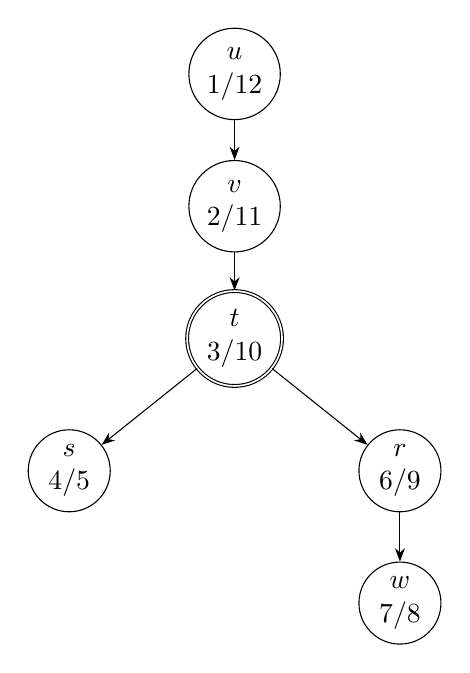
\begin{tikzpicture}[x=1.5cm,y=1.4cm]
\node[v](u)at(0,0){$u$\\$1/12$};\node[v](v)at(0,-1.2){$v$\\$2/11$};
\node[bf](t)at(0,-2.4){$t$\\$3/10$};\node[v](s)at(-1.4,-3.6){$s$\\$4/5$};
\node[v](r)at(1.4,-3.6){$r$\\$6/9$};\node[v](w)at(1.4,-4.8){$w$\\$7/8$};
\foreach\a/\b in{u/v,v/t,t/s,t/r,r/w}\draw[arr](\a)--(\b);
\end{tikzpicture}\end{center}
Each pair is discovery/finish time. After $s$ finishes, DFS returns to $t$, which has an unvisited neighbor $r$. Thus $\boxed{t}$ is the backtracking branch point where a new route starts. The dead ends are $s$ and $w$.

The complete return sequence is
\[
s\rightsquigarrow t,\quad w\rightsquigarrow r\rightsquigarrow t\rightsquigarrow v\rightsquigarrow u.
\]
If ``backtrack nodes'' means all nodes receiving a recursive return, they are $t,r,v,u$; if it means a return point that starts a different unvisited branch, it is $t$ alone. This distinction is also used in DFS2 and DFS3.

The non-tree edges $(s,u)$ and $(w,v)$ connect descendants to ancestors, so they are back edges in this undirected DFS. An undirected graph has only tree and back edges under the usual DFS edge classification.

\newpage
\question{DFS2 (p.\ 3)}{Discovery and finish times}
\textbf{Reading the supplied tree literally.} The left diagram contains two occurrences of $D$. Label the one below $E$ as $D_1$ and the one directly below $A$ as $D_2$. Treating these as separate tree occurrences and visiting children left to right gives:
\begin{center}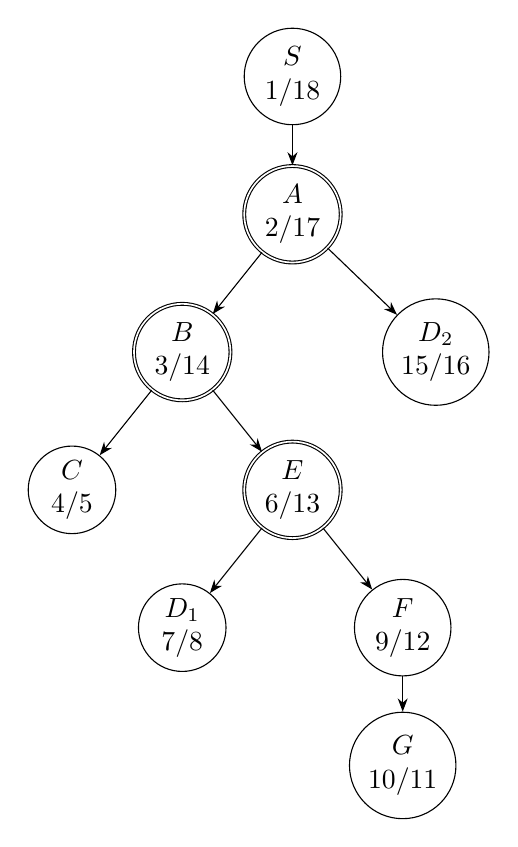
\begin{tikzpicture}[x=1.4cm,y=1.4cm]
\node[v](S)at(0,0){$S$\\$1/18$};\node[bf](A)at(0,-1.25){$A$\\$2/17$};
\node[bf](B)at(-1,-2.5){$B$\\$3/14$};\node[v](D2)at(1.3,-2.5){$D_2$\\$15/16$};
\node[v](C)at(-2,-3.75){$C$\\$4/5$};\node[bf](E)at(0,-3.75){$E$\\$6/13$};
\node[v](D1)at(-1,-5){$D_1$\\$7/8$};\node[v](F)at(1,-5){$F$\\$9/12$};\node[v](G)at(1,-6.25){$G$\\$10/11$};
\foreach\a/\b in{S/A,A/B,A/D2,B/C,B/E,E/D1,E/F,F/G}\draw[arr](\a)--(\b);
\end{tikzpicture}\end{center}
The branch points at which DFS returns and begins another branch are
\[
C\rightsquigarrow\boxed{B}\to E,\quad D_1\rightsquigarrow\boxed{E}\to F,
\quad G\rightsquigarrow F\rightsquigarrow E\rightsquigarrow B\rightsquigarrow\boxed{A}\to D_2.
\]
The dead-end occurrences are $C,D_1,G,D_2$. Every internal node eventually receives a recursive return: $S,A,B,E,F$.

\textbf{If the intended algorithm is graph DFS on the right-hand graph:} $D$ is discovered only once, below $E$. The later edge $A$--$D$ does not create another tree node. The corrected timestamps are
\[
S:1/16,\ A:2/15,\ B:3/14,\ C:4/5,\ E:6/13,\ D:7/8,\ F:9/12,\ G:10/11.
\]
Only $B$ and $E$ start a new unvisited branch after backtracking. The two readings are separated because the supplied tree repeats the graph vertex $D$.

\newpage
\question{DFS3 (p.\ 4)}{Continue after the dead end}
Use $(r,c)$ for row and column. Keep all previously visited nodes marked. The question does not fix the order of the remaining unvisited neighbors, so the following is one valid continuation.

\textbf{First backtracking point.} At $(3,2)$, all neighbors have already been visited. Backtrack along the active DFS stack:
\[
(3,2)\rightsquigarrow(2,2)\rightsquigarrow(1,2)\rightsquigarrow(1,1)
\rightsquigarrow(2,1)\rightsquigarrow(3,1)\rightsquigarrow(4,1).
\]
The first node with an unvisited neighbor is $\boxed{bf_1=(4,1)}$. Continue into the lower-left pocket:
\[
(4,1)\to(5,1)\to(6,1)\to(6,2).
\]
At $(6,2)$, its neighbors $(6,1),(5,2),(6,3)$ are all visited, so it is another dead end.

\textbf{Second backtracking point.} Return via
\[
(6,2)\rightsquigarrow(6,1)\rightsquigarrow(5,1)\rightsquigarrow(4,1)\rightsquigarrow(4,2).
\]
Now $\boxed{bf_2=(4,2)}$ has the unvisited neighbor $(4,3)$. Continue:
\[
(4,2)\to(4,3)\to(4,4)\to\boxed{(5,4)}.
\]
The goal is reached, so stop.

\begin{center}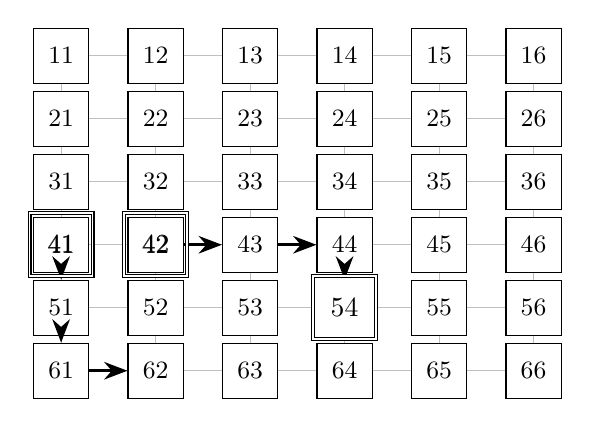
\begin{tikzpicture}[x=1.2cm,y=0.8cm]
\foreach\r in{1,...,6}\foreach\c in{1,...,6}{\node[draw,rectangle,minimum size=7mm,fill=white](n\r\c)at(\c,-\r){\small\r\c};}
\foreach\r in{1,...,6}\foreach\c in{1,...,5}{\pgfmathtruncatemacro{\d}{\c+1}\draw[gray!50](n\r\c)--(n\r\d);}
\foreach\r in{1,...,5}\foreach\c in{1,...,6}{\pgfmathtruncatemacro{\d}{\r+1}\draw[gray!50](n\r\c)--(n\d\c);}
\foreach\a/\b in{41/51,51/61,61/62,42/43,43/44,44/54}\draw[arr,very thick](n\a)--(n\b);
\node[draw,rectangle,minimum size=8mm,double]at(n41){41};\node[draw,rectangle,minimum size=8mm,double]at(n42){42};
\node[draw,rectangle,minimum size=8mm,double,fill=white]at(n54){54};
\end{tikzpicture}\end{center}
The arrows show only newly explored edges. Double boxes mark $bf_1=41$, $bf_2=42$, and the goal 54. The final start-to-goal stack is
\begin{align*}
33\to23\to13\to14\to15\to25\to35\to45\to55\\
\to65\to64\to63\to53\to52\to42\to43\to44\to54.
\end{align*}
Here $33$ means $(3,3)$, and similarly for the other labels. The dead-end side branches are removed from the final path.

\newpage
\question{DFS4 (p.\ 5)}{DFS starting from $v$}
Start with $v$. After its component finishes, scan the remaining vertices alphabetically. Use alphabetical adjacency lists throughout.
\begin{center}\begin{tabular}{c|l@{\qquad}c|l}\toprule
Vertex&Outgoing neighbors&Vertex&Outgoing neighbors\\\midrule
$q$&$s,t,w$&$r$&$u,y$\\$s$&$v$&$t$&$x,y$\\$u$&$y$&$v$&$w$\\$w$&$s$&$x$&$z$\\$y$&$q$&$z$&$x$\\\bottomrule\end{tabular}\end{center}
The discovery order is
\[
\boxed{v,w,s,q,t,x,z,y,r,u}.
\]
The resulting DFS forest has three roots, $v,q,r$:
\begin{center}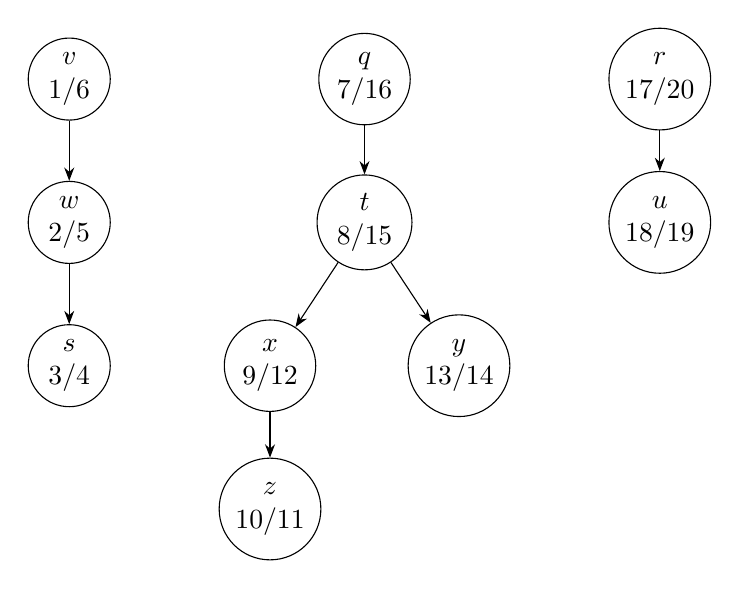
\begin{tikzpicture}[x=1.5cm,y=1.4cm]
\node[v](v)at(0,0){$v$\\$1/6$};\node[v](w)at(0,-1.3){$w$\\$2/5$};\node[v](s)at(0,-2.6){$s$\\$3/4$};
\node[v](q)at(2.5,0){$q$\\$7/16$};\node[v](t)at(2.5,-1.3){$t$\\$8/15$};
\node[v](x)at(1.7,-2.6){$x$\\$9/12$};\node[v](y)at(3.3,-2.6){$y$\\$13/14$};\node[v](z)at(1.7,-3.9){$z$\\$10/11$};
\node[v](r)at(5,0){$r$\\$17/20$};\node[v](u)at(5,-1.3){$u$\\$18/19$};
\foreach\a/\b in{v/w,w/s,q/t,t/x,x/z,t/y,r/u}\draw[arr](\a)--(\b);
\end{tikzpicture}\end{center}
Finish order: $s,w,v,z,x,y,t,q,u,r$. The non-tree edges are:
\begin{itemize}[nosep]
\item Back edges: $s\to v$, $z\to x$, $y\to q$.
\item Cross edges: $q\to s$, $q\to w$, $u\to y$, $r\to y$.
\end{itemize}
Only $v,w,s$ are reachable from the initial root $v$; the outer DFS loop is needed to visit the rest.

\newpage
\question{DFS5 (p.\ 6)}{Topological ordering}
One valid topological ordering is
\[
\boxed{p,n,o,s,m,r,y,v,x,w,z,u,q,t}.
\]
It can be obtained by running DFS with alphabetical outer and adjacency order, then reversing the finish order. Every directed edge goes from an earlier vertex to a later vertex:
\begin{center}\begin{tabular}{c|l}\toprule
Vertex&Its outgoing neighbors, all later in the ordering\\\midrule
$p$&$o,s,z$\\$n$&$o,q,u$\\$o$&$r,s,v$\\$s$&$r$\\$m$&$q,r,x$\\$r$&$u,y$\\$y$&$v$\\$v$&$w,x$\\$w$&$z$\\$u$&$t$\\$q$&$t$\\\bottomrule\end{tabular}\end{center}
The vertices $t,x,z$ have no outgoing edges. This check includes every edge in the supplied graph. A DAG may have several valid topological orders; the displayed order is one of them.

\newpage
\question{Dijkstra1 (p.\ 7)}{Complete the shortest-path calculation}
The source is $a$. The supplied edge $b$--$h$ has weight \textbf{1}; use this value rather than the weight in a different textbook version of this graph. Set $d(a)=0$ and every other tentative distance to $\infty$.

Use the relaxation rule $d(v)\gets\min\{d(v),d(u)+w(u,v)\}$. At each step, settle the unsettled vertex with the smallest tentative distance. Break the $c/i$ tie alphabetically.
\begin{center}\small\begin{tabular}{c|c|rrrrrrrrr}\toprule
Step&Settled&$a$&$b$&$h$&$g$&$f$&$c$&$i$&$e$&$d$\\\midrule
0&--&0&$\infty$&$\infty$&$\infty$&$\infty$&$\infty$&$\infty$&$\infty$&$\infty$\\
1&$a$&0&4&8&$\infty$&$\infty$&$\infty$&$\infty$&$\infty$&$\infty$\\
2&$b$&0&4&5&$\infty$&$\infty$&12&$\infty$&$\infty$&$\infty$\\
3&$h$&0&4&5&6&$\infty$&12&12&$\infty$&$\infty$\\
4&$g$&0&4&5&6&8&12&12&$\infty$&$\infty$\\
5&$f$&0&4&5&6&8&12&12&18&22\\
6&$c$&0&4&5&6&8&12&12&18&19\\
7&$i$&0&4&5&6&8&12&12&18&19\\
8&$e$&0&4&5&6&8&12&12&18&19\\
9&$d$&0&4&5&6&8&12&12&18&19\\\bottomrule
\end{tabular}\normalsize\end{center}
The important updates after the illustrated prefix are:
\begin{align*}
d(g)&=d(h)+1=6,& d(i)&=d(h)+7=12,\\
d(f)&=d(g)+2=8,& d(e)&=d(f)+10=18,\\
d(d)&=d(f)+14=22\quad\text{initially},&&\\
d(d)&=\min(22,d(c)+7)=\min(22,19)=19.&&
\end{align*}
Settling $i,e,d$ causes no further improvements. The final shortest-path tree is:
\begin{center}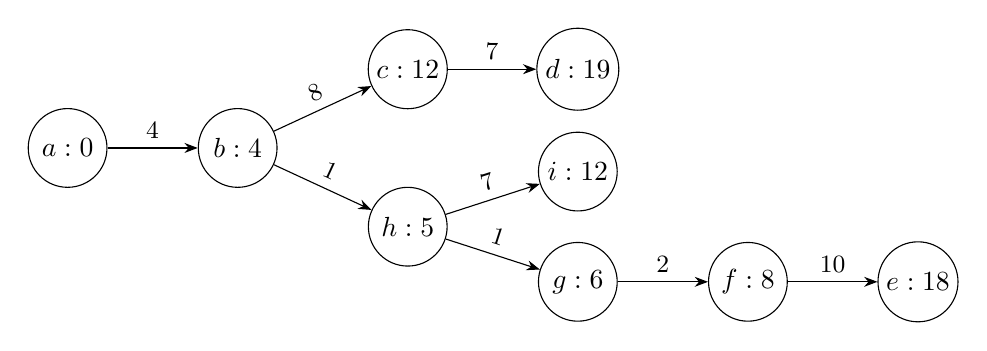
\begin{tikzpicture}[x=1.2cm,y=1cm]
\node[v](a)at(0,0){$a:0$};\node[v](b)at(1.8,0){$b:4$};\node[v](c)at(3.6,1){$c:12$};\node[v](d)at(5.4,1){$d:19$};
\node[v](h)at(3.6,-1){$h:5$};\node[v](i)at(5.4,-0.3){$i:12$};\node[v](g)at(5.4,-1.7){$g:6$};\node[v](f)at(7.2,-1.7){$f:8$};\node[v](e)at(9,-1.7){$e:18$};
\foreach\a/\b/\w in{a/b/4,b/c/8,c/d/7,b/h/1,h/i/7,h/g/1,g/f/2,f/e/10}\draw[arr](\a)--node[above,sloped]{\small\w}(\b);
\end{tikzpicture}\end{center}
Each node label gives the vertex and its final distance. The source-to-vertex paths are read directly from this tree.

\newpage
\question{AStar1 (p.\ 8)}{A* with $h(B)=16$}
Let $g(n)$ be the best known path cost from $A$, and let $f(n)=g(n)+h(n)$. The heuristic values are
\[
\begin{array}{c|rrrrrrrrrr}
n&A&X&B&C&L&W&K&T&S&H\\\hline
h(n)&30&27&16&17&33&9&19&0&17&22
\end{array}
\]
Start with OPEN $=\{A\}$, $g(A)=0$, and $f(A)=30$. In the table, $n(g,f)$ denotes a queued node with its current $g$ and $f$ values. OPEN is shown in increasing $f$ order after each expansion.
\begin{center}\small\begin{tabular}{c|c|>{\raggedright\arraybackslash}p{6.4cm}|>{\raggedright\arraybackslash}p{4.4cm}}\toprule
Step&Pop&Calculations&OPEN after step\\\midrule
1&$A$&$g(X)=0+17=17$, $f(X)=17+27=44$&$X(17,44)$\\
2&$X$&$g(B)=17+16=33$, $f(B)=49$; $g(C)=17+11=28$, $f(C)=45$&$C(28,45)$, $B(33,49)$\\
3&$C$&$g(W)=28+11=39$, $f(W)=48$; $g(L)=28+20=48$, $f(L)=81$&$W(39,48)$, $B(33,49)$, $L(48,81)$\\
4&$W$&$g(T)=39+9=48$, $f(T)=48$; $g(K)=39+10=49$, $f(K)=68$; candidate $g(B)=39+12=51>33$, so keep $B$ unchanged.&$T(48,48)$, $B(33,49)$, $K(49,68)$, $L(48,81)$\\
5&$T$&$T$ is popped as the lowest-$f$ node. It is the goal, so stop.&$B(33,49)$, $K(49,68)$, $L(48,81)$\\\bottomrule\end{tabular}\normalsize\end{center}
The CLOSED sequence is $A,X,C,W,T$. Edges back to previously processed nodes do not improve their costs in this run. Follow the parent pointers:
\[
\boxed{A\to X\to C\to W\to T},\qquad
\boxed{17+11+11+9=48}.
\]
\begin{center}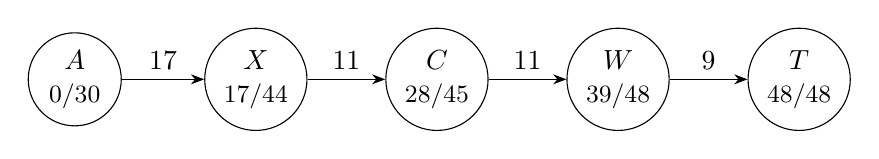
\begin{tikzpicture}[x=2.3cm]
\foreach\n/\x/\g/\f in{A/0/0/30,X/1/17/44,C/2/28/45,W/3/39/48,T/4/48/48}{\node[v](\n)at(\x,0){$\n$\\\small$\g/\f$};}
\foreach\a/\b/\w in{A/X/17,X/C/11,C/W/11,W/T/9}\draw[arr](\a)--node[above]{\w}(\b);
\end{tikzpicture}\end{center}
The pair under each node is $g/f$. The goal is tested when it is popped, not immediately when it is first generated.

\newpage
\question{AStar2 (p.\ 9)}{Change $h(B)$ from 16 to 6}
Use the same initialization and relaxation rule, with $h(B)=6$. Whenever a better route to a node already in OPEN is found, update its $g$, $f$, and parent, and restore the priority order.
\begin{center}\small\begin{tabular}{c|c|>{\raggedright\arraybackslash}p{6.2cm}|>{\raggedright\arraybackslash}p{4.6cm}}\toprule
Step&Pop&Calculations&OPEN after step\\\midrule
1&$A$&$g(X)=17$, $f(X)=44$&$X(17,44)$\\
2&$X$&$g(B)=33$, $f(B)=33+6=39$; $g(C)=28$, $f(C)=45$&$B(33,39)$, $C(28,45)$\\
3&$B$&$g(W)=33+12=45$, $f(W)=54$; $g(T)=33+17=50$, $f(T)=50$; $g(S)=33+7=40$, $f(S)=57$&$C(28,45)$, $T(50,50)$, $W(45,54)$, $S(40,57)$\\
4&$C$&Candidate $g(W)=28+11=39<45$: update $W$, $f(W)=48$, parent$(W)=C$. Also $g(L)=48$, $f(L)=81$.&$W(39,48)$, $T(50,50)$, $S(40,57)$, $L(48,81)$\\
5&$W$&Candidate $g(T)=39+9=48<50$: update $T$, $f(T)=48$, parent$(T)=W$. Also $g(K)=49$, $f(K)=68$. Candidate $g(B)=51>33$ is discarded.&$T(48,48)$, $S(40,57)$, $K(49,68)$, $L(48,81)$\\
6&$T$&Goal popped; stop.&$S(40,57)$, $K(49,68)$, $L(48,81)$\\\bottomrule\end{tabular}\normalsize\end{center}
Thus the correct A* calculation still returns
\[
\boxed{A\to X\to C\to W\to T\text{ with cost }48}.
\]
The expansion order changes to $A,X,B,C,W,T$, but the optimal path does not.

\textbf{What can go wrong?} If an implementation refuses to update a node already in OPEN, then after expanding $C$, $W$ incorrectly remains at $g=45,f=54$. It next pops $T$ with cost 50 and returns $A\to X\to B\to T$, which is suboptimal. Similarly, stopping when $T$ is first generated is incorrect. Successors need cost relaxation, not merely insertion or a visited test.

\textbf{Admissibility and consistency.} Both 16 and 6 underestimate the true remaining cost from $B$, which is 17, so both are admissible. However, the new heuristic is inconsistent, since
\[
h(X)=27>16+h(B)=22,\qquad h(S)=17>7+h(B)=13.
\]
For general graphs with an admissible but inconsistent heuristic, a CLOSED node must be reopened when a strictly better $g$ is found. In \emph{this particular run}, no CLOSED node receives a better cost: the necessary corrections concern $W$ and $T$ while they are still in OPEN.

\newpage
\question{AStar3 (p.\ 10)}{Shortest paths among polygonal obstacles}
\textbf{(a) Number of states.} If a state is an arbitrary collision-free position $(x,y)$ in the plane, there are \emph{uncountably infinitely many} states. The coordinates vary continuously; the drawing is not a finite grid. There are also infinitely many possible continuous paths to the goal.

An equivalent finite shortest-path search can use the visibility graph: keep only $S$, $G$, and polygon vertices, connecting pairs that can see one another without crossing an obstacle interior. The seven pictured obstacles have
\[
5+3+4+4+4+3+6=29\text{ vertices}.
\]
Including $S$ and $G$ gives $\boxed{31}$ visibility-graph vertices. The continuous state space and this reduced search graph are different representations; 31 is not the number of all physical positions.

\textbf{(b) Why can the shortest path follow polygon boundaries?} Between two fixed points in free space, a straight segment is shortest. A bend strictly inside free space can be replaced locally by a straight chord, shortening the path. A non-collinear bend at the interior of a straight obstacle edge can also be straightened within the free half-plane. Therefore, essential direction changes occur at obstacle vertices.

A shortest path is consequently made of straight segments joining $S$, $G$, and some obstacle vertices. Some segments can coincide with polygon edges, while others cross free space between visible vertices. It is not necessary for every segment of the path to lie on an obstacle boundary.

\begin{center}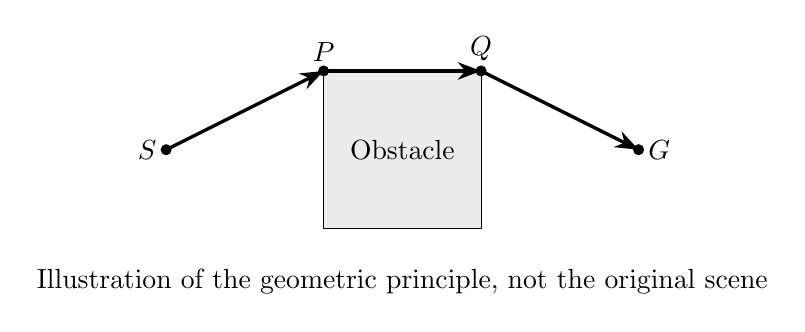
\begin{tikzpicture}[x=1cm,y=1cm]
\filldraw[fill=gray!15] (2,0)rectangle(4,2);
\coordinate(S)at(0,1);\coordinate(G)at(6,1);\coordinate(P)at(2,2);\coordinate(Q)at(4,2);
\draw[very thick,arr](S)--(P);\draw[very thick,arr](P)--(Q);\draw[very thick,arr](Q)--(G);
\fill(S)circle(2pt)node[left]{$S$};\fill(G)circle(2pt)node[right]{$G$};\fill(P)circle(2pt)node[above]{$P$};\fill(Q)circle(2pt)node[above]{$Q$};
\node at(3,1){Obstacle};\node[below]at(3,-0.4){Illustration of the geometric principle, not the original scene};
\end{tikzpicture}\end{center}
Assume a point robot, Euclidean path length, and that travel along obstacle boundaries is allowed. If contact is forbidden, boundary-hugging paths give the limiting infimum and can be approximated with arbitrarily small clearance.
\end{document}
